\documentclass[aspectratio=169]{beamer}

\usepackage{graphicx}
\usepackage{tcolorbox}

\usetheme{Boadilla}

\title{Forecasting Service Metrics - Linear Regression}
\subtitle{EP2420 Network Analytics}
\author{André Silva}
\date{December 07, 2020}

\begin{document}
\begin{frame}
    \titlepage
\end{frame}

\begin{frame}
    \frametitle{Previously}

    \begin{center}
        Build a model 
        \[M({\theta}) : x \rightarrow ŷ\]
        by minimizing
        \[\mathcal{L}({M(\theta,x^{(t)}),y^{(t)}})\]
        with respect to $\theta$, given the samples $(x^{(t)},y^{(t)})$ $t=1,\ldots,m$
    \end{center}
\end{frame}

\begin{frame}
    \frametitle{Objective}

    \begin{center}
        Build a model 
        \[M({\theta,h,l}) : [x_{-l},\ldots,x_{0}] \rightarrow [ŷ_{0},\ldots,ŷ_{h}]\]
        by minimizing
        \[\mathcal{L}({M(\theta,x^{(t)}),y^{(t)}})\]
        with respect to $\theta$, given the samples $(x^{(t)},y^{(t)})$ $t=1,\ldots,m$
    \end{center}
\end{frame}

\begin{frame}
    \frametitle{Transforming Dataset}

    \begin{enumerate}
        \item Standardize by column
        \item Remove outliers
        \item Tree-based feature selection, to extract top 16 features
        \item Generate pairs of sequences $([x^{(t-l)},\lodts,x^{(t)}],[y^{(t)},\ldots,y^{(t+h)}])$
    \end{enumerate}
\end{frame}

\begin{frame}
    \frametitle{Linear Regressors}
    \begin{figure}[h!]
        \centering
        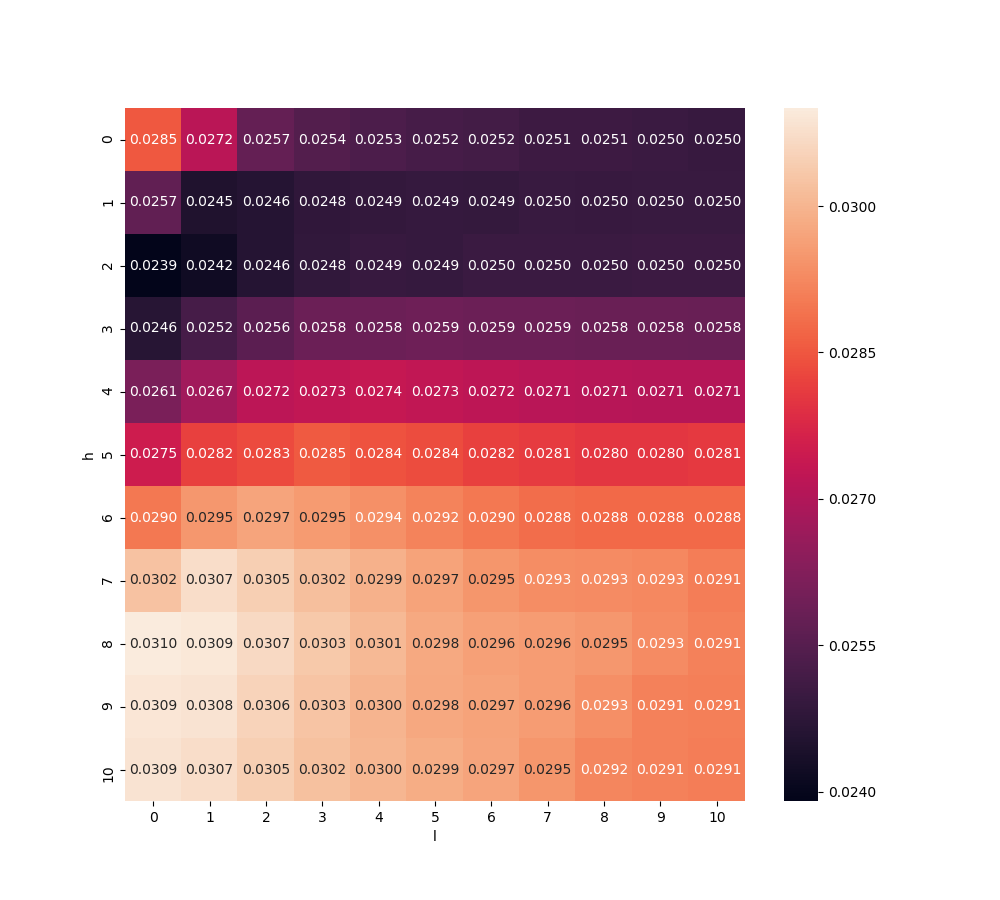
\includegraphics[width=\textwidth,height=0.75\textheight,keepaspectratio]{../result/project2/nmae_heatmap.png}
        \caption{Heat-map of \textsc{NMAE} for each Linear Regressor with $l\in\{0,\ldots,10\}$ when predicting $y^{(t+h)}$}
    \end{figure}
\end{frame}

\end{document}
